%%% Hlavní soubor. Zde se definují základní parametry a odkazuje se na ostatní části. %%%

%% Verze pro jednostranný tisk:
% Okraje: levý 40mm, pravý 25mm, horní a dolní 25mm
% (ale pozor, LaTeX si sám přidává 1in)
\documentclass[12pt,a4paper]{report}
\setlength\textwidth{145mm}
\setlength\textheight{247mm}
\setlength\oddsidemargin{15mm}
\setlength\evensidemargin{15mm}
\setlength\topmargin{0mm}
\setlength\headsep{0mm}
\setlength\headheight{0mm}
% \openright zařídí, aby následující text začínal na pravé straně knihy
\let\openright=\clearpage

%% Pokud tiskneme oboustranně:
% \documentclass[12pt,a4paper,twoside,openright]{report}
% \setlength\textwidth{145mm}
% \setlength\textheight{247mm}
% \setlength\oddsidemargin{15mm}
% \setlength\evensidemargin{0mm}
% \setlength\topmargin{0mm}
% \setlength\headsep{0mm}
% \setlength\headheight{0mm}
% \let\openright=\cleardoublepage

%% Použité kódování znaků: obvykle latin2, cp1250 nebo utf8:
\usepackage[utf8]{inputenc}

%% Ostatní balíčky
\usepackage{graphicx}
\usepackage{amsthm}

\usepackage[english]{babel}
\usepackage{blindtext}
\usepackage[labelfont={small,bf},textfont={small,it}]{caption}
\usepackage{verbatim}
\usepackage{color}
\usepackage{graphicx}
\usepackage{amsmath}
\usepackage{acronym}
\usepackage{todonotes}
\newcommand{\BLIND}[0]{{\color{red}\blindtext}}
\newcommand{\TODO}[1]{\smallskip\todo[inline,color=red!30,size=\footnotesize]{\sf \textbf{TODO:} #1}}
\newcommand{\IDEA}[1]{\smallskip\todo[inline,color=yellow!30,size=\footnotesize]{\sf \textbf{IDEA:} #1}}
\newcommand{\TODOIMG}[2]{
  \begin{figure}[htb]
    \centering
    \includegraphics[width=0.95\textwidth]{./img/todo.pdf}

    \caption{#2}
    \label{#1}
  \end{figure}
}

%% Balíček hyperref, kterým jdou vyrábět klikací odkazy v PDF,
%% ale hlavně ho používáme k uložení metadat do PDF (včetně obsahu).
%% POZOR, nezapomeňte vyplnit jméno práce a autora.
\usepackage[unicode]{hyperref}   % Musí být za všemi ostatními balíčky
\hypersetup{pdftitle=Development of a cloud platform for automatic speech recognition}
\hypersetup{pdfauthor=Ondřej Klejch}

%%% Drobné úpravy stylu

% Tato makra přesvědčují mírně ošklivým trikem LaTeX, aby hlavičky kapitol
% sázel příčetněji a nevynechával nad nimi spoustu místa. Směle ignorujte.
\makeatletter
\def\@makechapterhead#1{
  {\parindent \z@ \raggedright \normalfont
   \Huge\bfseries \thechapter. #1
   \par\nobreak
   \vskip 20\p@
}}
\def\@makeschapterhead#1{
  {\parindent \z@ \raggedright \normalfont
   \Huge\bfseries #1
   \par\nobreak
   \vskip 20\p@
}}
\makeatother

% Toto makro definuje kapitolu, která není očíslovaná, ale je uvedena v obsahu.
\def\chapwithtoc#1{
\chapter*{#1}
\addcontentsline{toc}{chapter}{#1}
}

\begin{document}

% Trochu volnější nastavení dělení slov, než je default.
\lefthyphenmin=2
\righthyphenmin=2

%%% Titulní strana práce

\pagestyle{empty}
\begin{center}

\large

Charles University in Prague

\medskip

Faculty of Mathematics and Physics

\vfill

{\bf\Large MASTER THESIS}

\vfill

\centerline{\mbox{\includegraphics[width=60mm]{./img/logo.eps}}}

\vfill
\vspace{5mm}

{\LARGE Ondřej Klejch}

\vspace{15mm}

% Název práce přesně podle zadání
{\LARGE\bfseries Development of a cloud platform for automatic speech recognition}

\vfill

% Název katedry nebo ústavu, kde byla práce oficiálně zadána
% (dle Organizační struktury MFF UK)
Institute of Formal and Applied Linguistics

\vfill

\begin{tabular}{rl}

Supervisor of the master thesis: & Mgr. Ing. Filip Jurčíček Ph.D. \\
\noalign{\vspace{2mm}}
Study programme: & Informatics \\
\noalign{\vspace{2mm}}
Specialization: & Theoretical Computer Science \\
\end{tabular}

\vfill

% Zde doplňte rok
Prague 2015

\end{center}

\newpage

%%% Následuje vevázaný list -- kopie podepsaného "Zadání diplomové práce".
%%% Toto zadání NENÍ součástí elektronické verze práce, nescanovat.

%%% Na tomto místě mohou být napsána případná poděkování (vedoucímu práce,
%%% konzultantovi, tomu, kdo zapůjčil software, literaturu apod.)

\openright

\noindent
First of all, I would like to thank my supervisor, Mgr. Ing. Filip Jurčíček Ph.D., for his guidance, invaluable advices and time he has invested in me.
Also, I would like to thank my colleagues Ing. Lukáš Žilka, Mgr. Ondřej Plátek and Mgr. Ondřej Dušek for their valuable insights.
Finally, I would like to thank all of my family for their support during my studies.

Access to computing and storage facilities owned by parties and projects contributing to the National Grid Infrastructure MetaCentrum,
  provided under the programme "Projects of Large Infrastructure for Research, Development, and Innovations" (LM2010005), is greatly appreciated.

\newpage

%%% Strana s čestným prohlášením k diplomové práci

\vglue 0pt plus 1fill

\noindent
I declare that I carried out this master thesis independently, and only with the cited
sources, literature and other professional sources.

\medskip\noindent
I understand that my work relates to the rights and obligations under the Act No.
121/2000 Coll., the Copyright Act, as amended, in particular the fact that the Charles
University in Prague has the right to conclude a license agreement on the use of this
work as a school work pursuant to Section 60 paragraph 1 of the Copyright Act.

\vspace{10mm}

\hbox{\hbox to 0.5\hsize{%
In ........ date ............
\hss}\hbox to 0.5\hsize{%
signature of the author
\hss}}

\vspace{20mm}
\newpage

%%% Povinná informační strana diplomové práce

\vbox to 0.5\vsize{
\setlength\parindent{0mm}
\setlength\parskip{5mm}

Název práce:
Development of a cloud platform for automatic speech recognition
% přesně dle zadání

Autor:
Ondřej Klejch

Katedra:  % Případně Ústav:
Ústav formální a aplikované lingvistiky
% dle Organizační struktury MFF UK

Vedoucí diplomové práce:
Mgr. Ing. Filip Jurčíček Ph.D., Ústav formální a aplikované lingvistiky
% dle Organizační struktury MFF UK, případně plný název pracoviště mimo MFF UK

Abstrakt:
Tato diplomová práce představuje cloudovou platformu pro automatické rozpoznávání řeči, CloudASR,
  která je postavena na systému pro rozpoznávání řeči Kaldi.
Platforma podporuje dávkový a online způsob rozpoznávání řeči
  a také obsahuje anotační prostředí pro přidávání přepisů k odeslaným nahrávkám.
Mezi klíčové vlastnosti této platformy patří škálovatelnost, přizpůsobitelnost a jednoduchý proces nasazení.
Provedená měření dokázala,
  že latence platformy je porovnatelná s latencí Google Speech API
  a přesnost přepisů na omezených doménách může být dokonce lepší.
Dále bylo ukázáno,
  že je platforma schopná zpracovat více než 1000 paralelních dotazů,
  pokud má dostatek výpočetních zdrojů.
% abstrakt v rozsahu 80-200 slov; nejedná se však o opis zadání diplomové práce

Klíčová slova:
cloud, Kaldi, ASR
% 3 až 5 klíčových slov

\vss}\nobreak\vbox to 0.49\vsize{
\setlength\parindent{0mm}
\setlength\parskip{5mm}

Title:
Development of a cloud platform for automatic speech recognition

Author:
Ondřej Klejch

Department:
Institute of Formal and Applied Linguistics
% dle Organizační struktury MFF UK v angličtině

Supervisor:
Mgr. Ing. Filip Jurčíček Ph.D., Institute of Formal and Applied Linguistics
% dle Organizační struktury MFF UK, případně plný název pracoviště
% mimo MFF UK v angličtině

Abstract:
This thesis presents a cloud platform for automatic speech recognition, CloudASR,
  built on top of Kaldi speech recognition toolkit.
The platform supports both batch and online speech recognition mode
  and it has an annotation interface for transcription of the submitted recordings.
The key features of the platform are scalability, customizability and easy deployment.
Benchmarks of the platform show
  that the platform achieves comparable performance with Google Speech API in terms of latency
  and it can achieve better accuracy on limited domains.
Furthermore, the benchmarks show that the platform is able to handle more than 1000 parallel requests given enough computational resources.


% abstrakt v rozsahu 80-200 slov v angličtině; nejedná se však o překlad
% zadání diplomové práce

Keywords:
cloud, Kaldi, ASR
% 3 až 5 klíčových slov v angličtině

\vss}

\newpage

%%% Strana s automaticky generovaným obsahem diplomové práce. U matematických
%%% prací je přípustné, aby seznam tabulek a zkratek, existují-li, byl umístěn
%%% na začátku práce, místo na jejím konci.

\openright
\pagestyle{plain}
\setcounter{page}{1}
\tableofcontents

%%% Jednotlivé kapitoly práce jsou pro přehlednost uloženy v samostatných souborech
\chapter*{Introduction}
\addcontentsline{toc}{chapter}{Introduction}

Speech is the most natural form of human communication.
In order to be able to talk with a computer,
  it is crucial to have a good Automatic Speech Recognition (ASR) system.
On one hand, there are several open-source ASR toolkits,
  however deployment of such toolkits requires substantial knowledge,
  which makes them difficult to use for common software developers.
On the other hand, there are a few web services that provide ASR,
  yet these web services do not solve all problems -
  either they are paid, closed-source or they are not customizable.
So \textbf{the first goal of the present thesis is to develop a cloud platform for ASR}
  that is easy to use both from user's and maintainer's point of view.

Although the quality of ASR systems is improving,
  these systems are still far from perfect.
One of the reasons is that the quality of ASR systems depends heavily on the amount of the training data,
  and there is not enough publicly available transcribed speech data for all languages.
By providing free ASR web service it is possible to collect vast amount of recordings
  that can be manually transcribed.
Consequently, \textbf{the second goal of the present thesis is to create an annotation interface}
  so that recordings obtained by CloudASR platform can be annotated and given back to the community.

The following text development and deployment of CloudASR platform and its annotation interface are described.
Chapter~1 introduces Automatic Speech Recognition theory and tools related to CloudASR.
In Chapter~2, tools used for CloudASR development and deployment are presented.
The implementation of CloudASR platform is described in Chapter~3.
Chapter~4 contains results of conducted benchmarks.
Finally, Chapter~5 concludes this thesis.

\chapter{Theoretical Background}
This chapter describes theory needed for the CloudASR platform.
It starts with \textbf{Automatic Speech Recognition} section,
  which introduces concepts such as acoustic models, language models or speech decoding.
Then, sections \textbf{Open-Source ASR Tools} and \textbf{Public ASR services} present technologies related to CloudASR.
Finally, this chapter ends with \textbf{Obtaining Manual Transcriptions} section,
  which shows how manual transcriptions can be obtained with crowd--sourcing.

\section{Automatic Speech Recognition}
The task of the automatic speech recognition system is to "pick the most likely word sequence $\widehat{W}$
  given the observed acoustic evidence A" \cite{frederick1997statistical}.
Therefore, speech recognition can be described as a following formula:

\begin{equation}
  \label{eq:1}
  \widehat{W} = \arg \max_{W} P(W|A)
\end{equation}

By using Bayes' formula of probability theory,
  right-hand side of the Equation~\ref{eq:1} can be rewritten in a following way:

\begin{equation}
 \widehat{W} = \arg \max_{W} \frac{P(A|W) P(W)}{P(A)}
\end{equation}

Since the numerator P(A) is constant regarding the maximization,
  it can be omitted to get the final equation:

\begin{equation}
  \label{eq:asr}
  \widehat{W} = \arg \max_{W} P(A|W) P(W)
\end{equation}

Then, the probability $P(A|W)$ is called acoustic model and the probability $P(W)$ is called language model.
In the sections \textbf{Acoustic Models} and \textbf{Language Models} computation of these probabilities will be described in more detail.
After that, \textbf{Speech Decoding} section will describe how the Formula~\ref{eq:asr} is used to find the desired word sequence.


\subsection{Acoustic Models}
\BLIND
\BLIND

Baum--Welch \cite{welch2003hidden}
Viterbi training \cite{franzini1990connectionist}

\subsection{Language Models}
The task of the language model $P(W)$ in speech recognition is
  to determine how likely are the sequences of words $w_1,\dots,w_m$ that sound alike
  by assigning a probability to each sequence.
Using the Bayes' rule, $P(W)$ can be seen as:

\begin{equation}
  P(W) = P(w_1,\dots,w_m) = \prod\limits_{i=1}^{m} P(w_i|w_1,\dots,w_{i-1})
\end{equation}

Since the probability $P(w_i|w_1,\dots,w_{i-1})$ has just too many arguments
  and the probability does not necessarily depends on the entire history,
  the history is put into equivalence classes $\phi(w_1,\dots,w_{i-1})$.
This results into the following formula:

\begin{equation}
  P(w_1,\dots,w_m) \approx \prod\limits_{i=1}^{m} P(w_i|\phi(w_1,\dots,w_{i_1}))
\end{equation}

Traditionally, n-gram language models,
  which use the following history equivalence classes $\phi(w_1,\dots,w_{i-1}) = w_{i-(n-1)},\dots,w_{i-1}$,
  are used in speech recognition tasks.
Thus, the n-gram language model becomes:

\begin{equation}
  P(w_1,\dots,w_m) \approx \prod\limits_{i=1}^{m} P(w_i|w_{i-(n-1)},\dots,w_{i-1})
\end{equation}

Where the probabilities $P(w_i|w_{i-(n-1)},\dots,w_{w-1})$ are estimated from the relative frequencies of n-grams in the training data with the following formula:
\begin{equation}
  \label{eq:2}
  P(w_i|w_{i-(n-1)},\dots,w_{i-1}) = \frac{c(w_{i-(n-1)},\dots,w_i)}{c(w_{i-(n-1)},\dots,w_{i-1})}
\end{equation}


Since the numerator of the Equation~\ref{eq:2} can be zero due to data sparsity problem,
  several smoothing techniques such as
  Jelinek--Mercer \cite{jelinek1980interpolated},
  Good--Turing \cite{gale1995good}
  or Kneser--Ney \cite{kneser1995improved} are often used to estimate the higher n-gram relative frequencies from the lower n-gram frequencies.

Recently, artificial neural networks have been also successfully used to tackle the data sparsity problem \cite{bengio2003neural}.
For instance, the recurrent neural network based language models yielded state-of-the-art results in terms of WER in speech recognition \cite{mikolov2010recurrent}.


\subsection{Speech Decoding}
\BLIND
\BLIND


\section{Open-Source ASR Tools}
In the following section some of the open-source ASR tools will be described.
Namely, \textbf{HTK}, \textbf{Julius}, \textbf{Kaldi} and \textbf{RWTH}.


\textbf{HTK} \cite{young1997htk} is the first toolkit, that will be described.
HTK is a toolkit for building and manipulating hidden Markov models.
It consists of a set of library modules and tools that provide sophisticated facilities for speech analysis, HMM training, testing and results analysis.
Furthermore, it supports HMMs using both continuous density mixture Gaussians and discrete distributions and can be used to build complex HMM systems.

The second toolkit is \textbf{Julius} \cite{lee2001julius}, high-performance large vocabulary speech recognition decoder,
  that can perform almost real-time decoding with 60k words in the vocabulary.
It supports statistical n-gram language model and rule-based grammars,
  as well as Hidden Markov Model (HMM) as an acoustic model
Julius can be also used with models trained for HTK toolkit.

Next described toolkit is \textbf{Kaldi} \cite{povey2011kaldi} -- a free, open-source toolkit for speech recognition written in C++.
Its speech recognition system is based on finite-state transducers
  and it supports modelling of arbitrary phonetic-context sizes,
  acoustic modelling with subspace Gaussian mixture models (SGMM)
  as well as standard Gaussian mixture models and deep neural networks,
  together with all commonly used linear and affine transforms.

Furthermore, there is also a Python wrapper for Kaldi called PyKaldi \cite{platek2014free},
  which supports the online speech recognition.
CloudASR uses PyKaldi as a default speech recognition system.

The last toolkit that will be described is \textbf{RWTH} \cite{rybach2009rwth},
  which is a publicly available speech recognition toolkit developed at Aachen University.
It includes state of the art speech recognition technology for acoustic model training and decoding.
Besides, its notable components are speaker adaptation,
  speaker adaptive training,
  unsupervised training,
  a finite state automata library,
  and an efficient tree search decoder.


\section{Public ASR services}
In addition to these open sources ASR toolkits
  there are also several web services that provide an API for speech recognition.
Some of these services will be described in the following section.

\textbf{Google Speech API} supports speech recognition for 39 languages and their dialects.
Its batch API, illustrated in Figure~\ref{fig:google-api}, is very simple and can be used for transcription of the wave or flac files.
Additionally,
  Google Speech API supports the online speech recognition mode through JavaScript class SpeechRecognition in Google Chrome web browser.\footnote{\url{https://www.google.com/intl/en/chrome/demos/speech.html}}

\begin{figure}[h]
  \verbatiminput{snippets/google-api.bash}

  \caption{An example of Google Speech API batch speech recognition mode request for a transcription of a recording in British English.}
  \label{fig:google-api}
\end{figure}


\textbf{Nuance Dragon NaturallySpeaking}\footnote{\url{http://www.nuance.com/for-developers/dragon/index.htm}}
  is the second provider of the API for speech recognition.
It provides software development kits for Windows and mobile applications.
It also has a version that can be deployed on a server and used as a API for other applications.


The last API provider that will be mentioned here is \textbf{wit.ai}\footnote{\url{https://wit.ai/}}.
It supports 11 languages via an API similar to Google Speech API, see Figure~\ref{fig:wit-ai-request} for an example,
  and in addition to speech recognition it also supports intent classification of the submitted recordings,
  see Figure~\ref{fig:wit-ai-response} for an exemplar response from the wit.ai.

\begin{figure}[h]
  \verbatiminput{snippets/google-api.bash}

  \caption{An example of wit.ai API request for a transcription of a recording.}
  \label{fig:wit-ai-request}
\end{figure}

\begin{figure}[h]
  \verbatiminput{snippets/wit-ai-response.json}

  \caption{An exemplar response from wit.ai API with a recording of a sentence: "I'm looking for a bar."}
  \label{fig:wit-ai-response}
\end{figure}


\section{Obtaining Manual Transcriptions}
A large amount of transcribed recordings is needed in order to train a good ASR system.
But a manual transcription of the recordings by professional transcribers is expensive and time demanding,
  typically, professional transcribers need 6 hours to transcribe 1 hour of speech data \cite{williams2011crowd}.
Furthermore, it is difficult to find enough professional transcribers to transcribe the required amount of speech data in short time.

Recently, it was shown that crowd-sourcing can be used for cheap, fast and good enough manual transcription of speech data \cite{novotney2010cheap}.
With crowd-sourcing, speech data is splitted into small chunks that are then transcribed by several non-professional transcribers.
Their transcriptions are then used to select the best transcription for the recording, for example with ROVER algorithm \cite{marge2010using}, and used for training of new ASR systems.
Also, transcriptions from non-professional transcribers are only $6\%$ worse than professional transcriptions
  and they cost only $\frac{1}{30}$ of the cost of professional transcription.
Finally, services like \textbf{Amazon Mechanical Turk}\footnote{\url{https://www.mturk.com}}
  or \textbf{CrowdFlower}\footnote{\url{http://www.crowdflower.com/}} already support the speech transcription tasks.

\chapter{Used Technologies}
\blindtext

\section{Platform}
\blindtext

\subsection{Mesos}
\blindtext

\subsection{Marathon}
\blindtext

\subsection{Docker}
\blindtext

\subsection{Jenkins-CI}
\blindtext


\section{Backend}
\blindtext

\subsection{ZeroMQ}
\blindtext

\subsection{Google Protocol Buffers}
\blindtext


\section{Frontend}
\blindtext

\subsection{WebAudio}
\blindtext

\subsection{Socket.io}
\blindtext


\chapter{Solution}
In this chapter I will describe the implementation of CloudASR,
  I will stress key design choices...

\section{Architecture}
The key requirement for the architecture of CloudASR is scalability.


Thus, the platform had to be designed from the very beginning to be able to run on many machines.


\IDEA{pre fork model, it is not possible to fork on demand}
\IDEA{not blocking architecture}

The architecture as described in Figure~\ref{fig:architecture} consists of several types of nodes,
  namely \textbf{API}, \textbf{Web}, \textbf{Master}, \textbf{Worker} and \textbf{Recordings Saver}.
These nodes communicate with each other by sending messages over ZeroMQ sockets,
  which allows each node to run on different machine.
\TODO{cite: Viewing control structures as patterns of passing messages}

\begin{figure}
  \centering
  \includegraphics[width=0.75\textwidth]{./img/architecture.pdf}

  \label{fig:architecture}
  \caption{\TODO{Architecture}}
\end{figure}

\IDEA{Master-Slave architecture, multiple workers}
\TODOIMG{fig:queue}{Queue architecture}

Each node was implemented with two main design patterns in mind, namely Dependency Injection and Factory Method.
Usage of these patterns together with message oriented architecture made possible to test the whole platform easily,
  because it enabled to pass test doubles into the nodes
  and then send fake messages needed to test a correct behaviour.
As a result, a typical unit test structure looks like a test in Figure~\ref{fig:unit-test}.
\TODO{cite: Inversion of control containers and the dependency injection pattern}
\TODO{cite: Design patterns: Abstraction and reuse of object-oriented design}

In addition to unit tests there are also integration tests,
  which test the factory methods that create production ready nodes,
  and end-to-end tests,
  which test that both batch and online recognition mode requests are handled correctly.
This test suite ensures that developers did not break anything
  and it also gives them confidence to change the code without fear.

\begin{figure}
  \verbatiminput{snippets/unit_test.py}

  \label{fig:unit-test}
  \caption{An example of unit test structure.}
  \TODO{add better caption}
\end{figure}


\subsection{API}
The main task of the API container is to forward requests from the clients to the workers.
The requests are either in form of HTTP POST for the batch mode or Socket.IO for the online mode.
The API is built on top of Flask framework with enabled asynchronous processing
  which allows single API container to process many parallel requests,
  because there are no blocking operations in the API container -
  it just receives requests from clients and forwards them via ZeroMQ to the workers.

\subsection{Web}
\IDEA{Mention Annotation Interface and Webdemo also link to screenshots}
\IDEA{Describe process of annotation}
CloudASR platform also has a web interface.
The web interface distinguishes between two types of user roles: administrators and users.
Administrators can browse all recordings with their transcriptions and manage workers descriptions.
Normal users are only allowed to add transcriptions to the recordings.

\TODOIMG{fig:annotation-interface}{Screen of the Annotation Interface}


Finally, the Web hosts a demo (See Figure~\ref{fig:webdemo}) of the CloudASR platform,
  through which users can try out different workers directly in their web browsers.
The demo has two modes, namely, dictation mode that only shows the best transcription of the recording
  and evaluation mode that also allows users to confirm that the recording is correct.

\TODOIMG{fig:webdemo}{Screen of a Web Demo}

\subsection{Master}
\IDEA{queue for every language}
The main task of the Master is to keep track about running workers and scheduling tasks to them.
The Master keeps track about running workers which send heartbeats with information about their state
  and when the Api asks for a worker address the master can return address of an available worker.

The workers can be in four different states:
  \textbf{started}, \textbf{waiting}, \textbf{working} and \textbf{not responding}.
  and it sends four different heartbeats:
  \textbf{started}, \textbf{waiting}, \textbf{working} and \textbf{finished}.
The worker starts in in the \textbf{started} state,
  after that it moves to the \textbf{waiting} state by sending the \textbf{waiting} heartbeat.
The worker remains in the waiting state until \textbf{the Master assings a tasks} to it,
  then it moves to the \textbf{working} state
  where it remains as long as it is working.
In the working state worker sends working heartbeats periodically,
  to inform the Master that it is working and it did not fail.
At the end of the task the Worker sends \textbf{finished} heartbeat
  and the Master changes the state of the Worker to the \textbf{working} state.

Additionally, when a worker crashes during the processing of the task and it gets restarted,
  it sends started heartbeat again,
  which informs the Master, that the worker was restarted and it adds it to the queue again.

When a worker does not send any heartbeat for 10 seconds,
  the master set the worker state to \textbf{not responding}.
But as soon as the worker sends any heartbeat,
  the master will set the worker to the appropriate state.

This whole process can be seen as a finite automaton illustrated in Figure~\ref{fig:worker-state}.

\begin{figure}
  \centering
  \includegraphics[width=0.75\textwidth]{./img/worker-state.pdf}

  \label{fig:worker-state}
  \caption{\TODO{Worker state transition diagram}}
\end{figure}

Unfortunately, the Master is a single point of failure of CloudASR platform.
When the Master stops working no speech recognition requests can be processed,
  because the API containers will not know to which worker they can forward the request.
But as soon as the Master starts working the platform should be available again.


\subsection{Worker}




\IDEA{VAD}
\IDEA{Kaldi}
\IDEA{Heartbeats}
\blindtext

\subsection{Deployment of New Kaldi Worker}
\blindtext

\subsection{Deployment of Arbitrary Worker}
\blindtext

\subsection{Recordings saver}
The main task of the Recordings saver is to save and serve recordings processed by workers.
When the worker finishes recognition it sends the recording with its n-best hypotheses to the Recording saver via ZeroMQ socket.
The saver saves the wave file to the filesystem and it save the n-best hypotheses to the database so that they can be used in the future.

\TODOIMG{fig:db-schema}{Database schema}



\section{Request Workflow}
\blindtext

\subsection{Batch Recognition}
\blindtext

\TODOIMG{fig:batch}{Batch Workflow}

\subsection{Online Recognition}
\blindtext

\TODOIMG{fig:online}{Online Workflow}



\section{Deployment}
\blindtext

\subsection{Single-Host Deployment}
Single-Host deployment allows users to run CloudASR directly on their machines.
The only dependency for running CloudASR is Docker.
After that it is possible to use prepared Makefile to run CloudASR by command \texttt{make run\_locally}.
The platform can stopped by command \texttt{make stop}.

The Makefile is prepared to run only one worker with English TownInfo model.
In order to run different worker users have to edit the Makefile, especially the name of the worker Docker image.

\TODO{don't use Makefile, use some python script with same interface for Multi-Host Deployment}

\subsection{Multi-Host Deployment}
\blindtext
\TODO{describe Mesos installation}
\TODO{insert example cloudasr.json configuration for the deployment}

\subsection{Scalability}
\blindtext

\subsection{Contiunous Integration \& Countinuous Delivery}
\blindtext


\section{Discussion}
\IDEA{Compare throughput of Queue vs Master-Slave, discuss options}
\IDEA{different architectures solving Harddisk bottleneck, Network bottleneck}

\chapter{Evaluation}
\blindtext

\section{CloudASR Platform Benchmarks}
\blindtext
\blindtext


\section{Batch Recognition Benchmark}
\blindtext
\blindtext

\section{Online Recognition Benchmark}
\blindtext
\blindtext


% Ukázka použití některých konstrukcí LateXu (odkomentujte, chcete-li)
% \include{example}

\chapter*{Conclusion}
\addcontentsline{toc}{chapter}{Conclusion}

Goals of this thesis were to develop a cloud platform for ASR, CloudASR,
  and an annotation interface for annotating speech data.
These goals were successfully accomplished and in several aspects even surpassed
  - in addition to original requirement to create batch recognition mode,
  online speech recognition mode was implemented.
In the following sections all achievements are summarized and
  at the end ideas for future work are proposed.

\section*{Cloud platform for ASR}
The first goal of this thesis was to develop a cloud platform for ASR, CloudASR,
  that would provide API for batch speech recognition mode of the submitted wave files.
This API is similiar to Google Speech API,
  which enables users to switch to CloudASR seamlessly.
In additition to that CloudASR provides an API for online speech recognition mode.
The CloudASR comes with a web demo,
  where the users can try out the online speech recognition mode with various languages.
Furthermore, the platform is scalable, customizable and easily deployable.


In terms of scalability,
  the platform is able to run both on single-machine and multi-machine setup
  and it allows to scale number of running workers according to users needs.
Additionally, the platform can run several API instances and load-balance between them.
The benchmarks show that the platform is able to handle more than 1000 parallel requests
  given enough computational resources.

The platform can handle requests for various languages at the same time.
Moreover, users can create workers for new languages using Pykaldi
  or they can even create workers for an arbitrary ASR systems
  if they provide a Python wrapper for that system.

Finally, CloudASR is easily deployable.
It uses Docker for creating and running application containers.
Therefore, users have to install only Docker for a single machine setup
  and a Mesos cluster for a multi machine setup.
Then it is possible to run the CloudASR platform with just one command.


\section*{Annotation interface}
The second goal of this thesis was to create an annotation interface for annotating submitted recordings.
Its responsibility is to collect and store obtained recordings together with their transcriptions.
Then users can rate transcriptions of the recordings
  or they can add their own transcriptions
  if they think that none transcription is correct.
The annotation interface allows administrators to choose golden transcription from several manual transcriptions
  that were obtained for the recording.
Additionally CloudASR also supports addition of manual transcriptions via external job at CrowdFlower.

\IDEA{Mention benefits of the thesis}

\section*{Future work}
\begin{itemize}
  \item
    Since manual transcription of recordings is expensive
      it would be good to make users transcribe only parts of the recordings
      in which ASR system wasn't confident enough \cite{sperber2014fly}.
    This idea could be used for both user transcription and CrowdFlower transcription.

  \item
    With manually transcribed recordings from CloudASR platform
      it is possible to continuously improve accuracy of the underlying ASR system
      by adapting the language model to the type of language that the users of the CloudASR really use.
    Thus CloudASR could provide an option to automatically update language model
      when a certain amount of new transcribed recordings was collected.

  \item
    Because running CloudASR platform is expensive in terms of costs for a server hosting,
      it would be good to optimize usage of individual workers
      so that spare workers are shut down when there is no need for them
      and new workers are started when the traffic arise.
    This can be achieved either by providing feedback control based systems \cite{janert2013feedback}
      or by using machine learning techniques \cite{gong2010press}.

  \item
    As CloudASR platform provides API for speech recognition,
      it could also be used for another speech related tasks like Language Identification, Speaker Identification, Voice Activity Detection, etc.

\end{itemize}




%%% Seznam použité literatury
%%% Seznam použité literatury je zpracován podle platných standardů. Povinnou citační
%%% normou pro diplomovou práci je ISO 690. Jména časopisů lze uvádět zkráceně, ale jen
%%% v kodifikované podobě. Všechny použité zdroje a prameny musí být řádně citovány.

\phantomsection
\addcontentsline{toc}{chapter}{\bibname}
\nocite{*}
\bibliography{citations}{}
\bibliographystyle{amsplain}

%\bibitem{lamport94}
%  {\sc Lamport,} Leslie.
%  \emph{\LaTeX: A Document Preparation System}.
%  2. vydání.
%  Massachusetts: Addison Wesley, 1994.
%  ISBN 0-201-52983-1.



%%% Tabulky v diplomové práci, existují-li.
% \chapwithtoc{List of Tables}

%%% Použité zkratky v diplomové práci, existují-li, včetně jejich vysvětlení.
\chapwithtoc{List of Abbreviations}
\begin{acronym}[TDMA]
  \acro{API} {Application Programming Interface}
  \acro{ASR} {Automatic Speech Recognition}
  \acro{DNN} {Deep Neural Network}
  \acro{HMM} {Hidden Markov Model}
  \acro{RTF} {Real Time Factor}
  \acro{SGMM} {Subspace Gaussian Mixture Model}
  \acro{VAD} {Voice Activity Detection}
  \acro{WER} {Word Error Rate}
\end{acronym}


%%% Přílohy k diplomové práci, existují-li (různé dodatky jako výpisy programů,
%%% diagramy apod.). Každá příloha musí být alespoň jednou odkazována z vlastního
%%% textu práce. Přílohy se číslují.

\appendix
\chapter{CD Content}

%\chapter{User Documentation}
%\chapter{Developer Documentation}
%\section{Installation}
%\section{Deployment}
%\section{Testing}


\openright
\end{document}
